%#! platex main.tex

\chapter{はじめに}
\label{cha:intro}

近年, 食事管理アプリにより, 食事の写真から食品やカロリなどの栄養素を自動で記録できるようになってきた. これらの技術は, 食事の写真から画像認識技術により, 食品を特定し, 栄養データを算出することがベースとなっている. 例えば, カロミル\footnote{健康管理アプリ、カロミルとは?|食事内容・日々の体重・運動量をアプリで簡単に記録~\url{https://www.calomeal.com/about-calomeal/}}は, iOS・Androidアプリとして提供されており, スマートフォンのカメラで食事の写真を撮るだけで, 食事の内容を解析し, 自動で摂取栄養素を記録することができる.

一方で, 健康的な食事を行う上で, 摂取栄養素だけでなく食べる順番やスピードを意識することは非常に重要である. 日本の学校教育では, 米やパンなどといった主食と, 汁物や飲料, おかずとを順序よく食べる方法「三角食べ」を推奨していた. 学術面においても, 食べる順番に重点をおいた食事指導の有効性については関西電力医学研究所の研究グループにより証明されており, 最初の5分間は食物繊維を含む食品やタンパク質や脂質を含む食品を食べ, その後, 炭水化物を含む食品を, 食物繊維を含む食品やタンパク質や脂質を含む食品と一緒に食べるよう指導すると, 体重の減量に影響を与えることを報告した\cite{yabe2019107450}. さらに, 糖尿病予防にも効果があり, 野菜から先に摂取すると, 米飯から先に摂取した場合と比較して食後の血糖値の上昇を抑えることができる\cite{tonyobyo53112}. また, 食べる速度についても, 早食いは肥満や糖尿病, 心臓に対して悪影響を及ぼすことが明らかになっている\cite{20249}\cite{beyond_willpower}. 一品ずつ集中して食べる「ばっかり食べ」や咀嚼をあまり行わない「早食い」をする子供に対して注意することは妥当であると言える.

%%%%%%%%%%%%%%%%%%%%%%%%%%%%%%%%%%%%%%%%%%%%%%%%
\begin{figure}[t]
  \begin{center}
    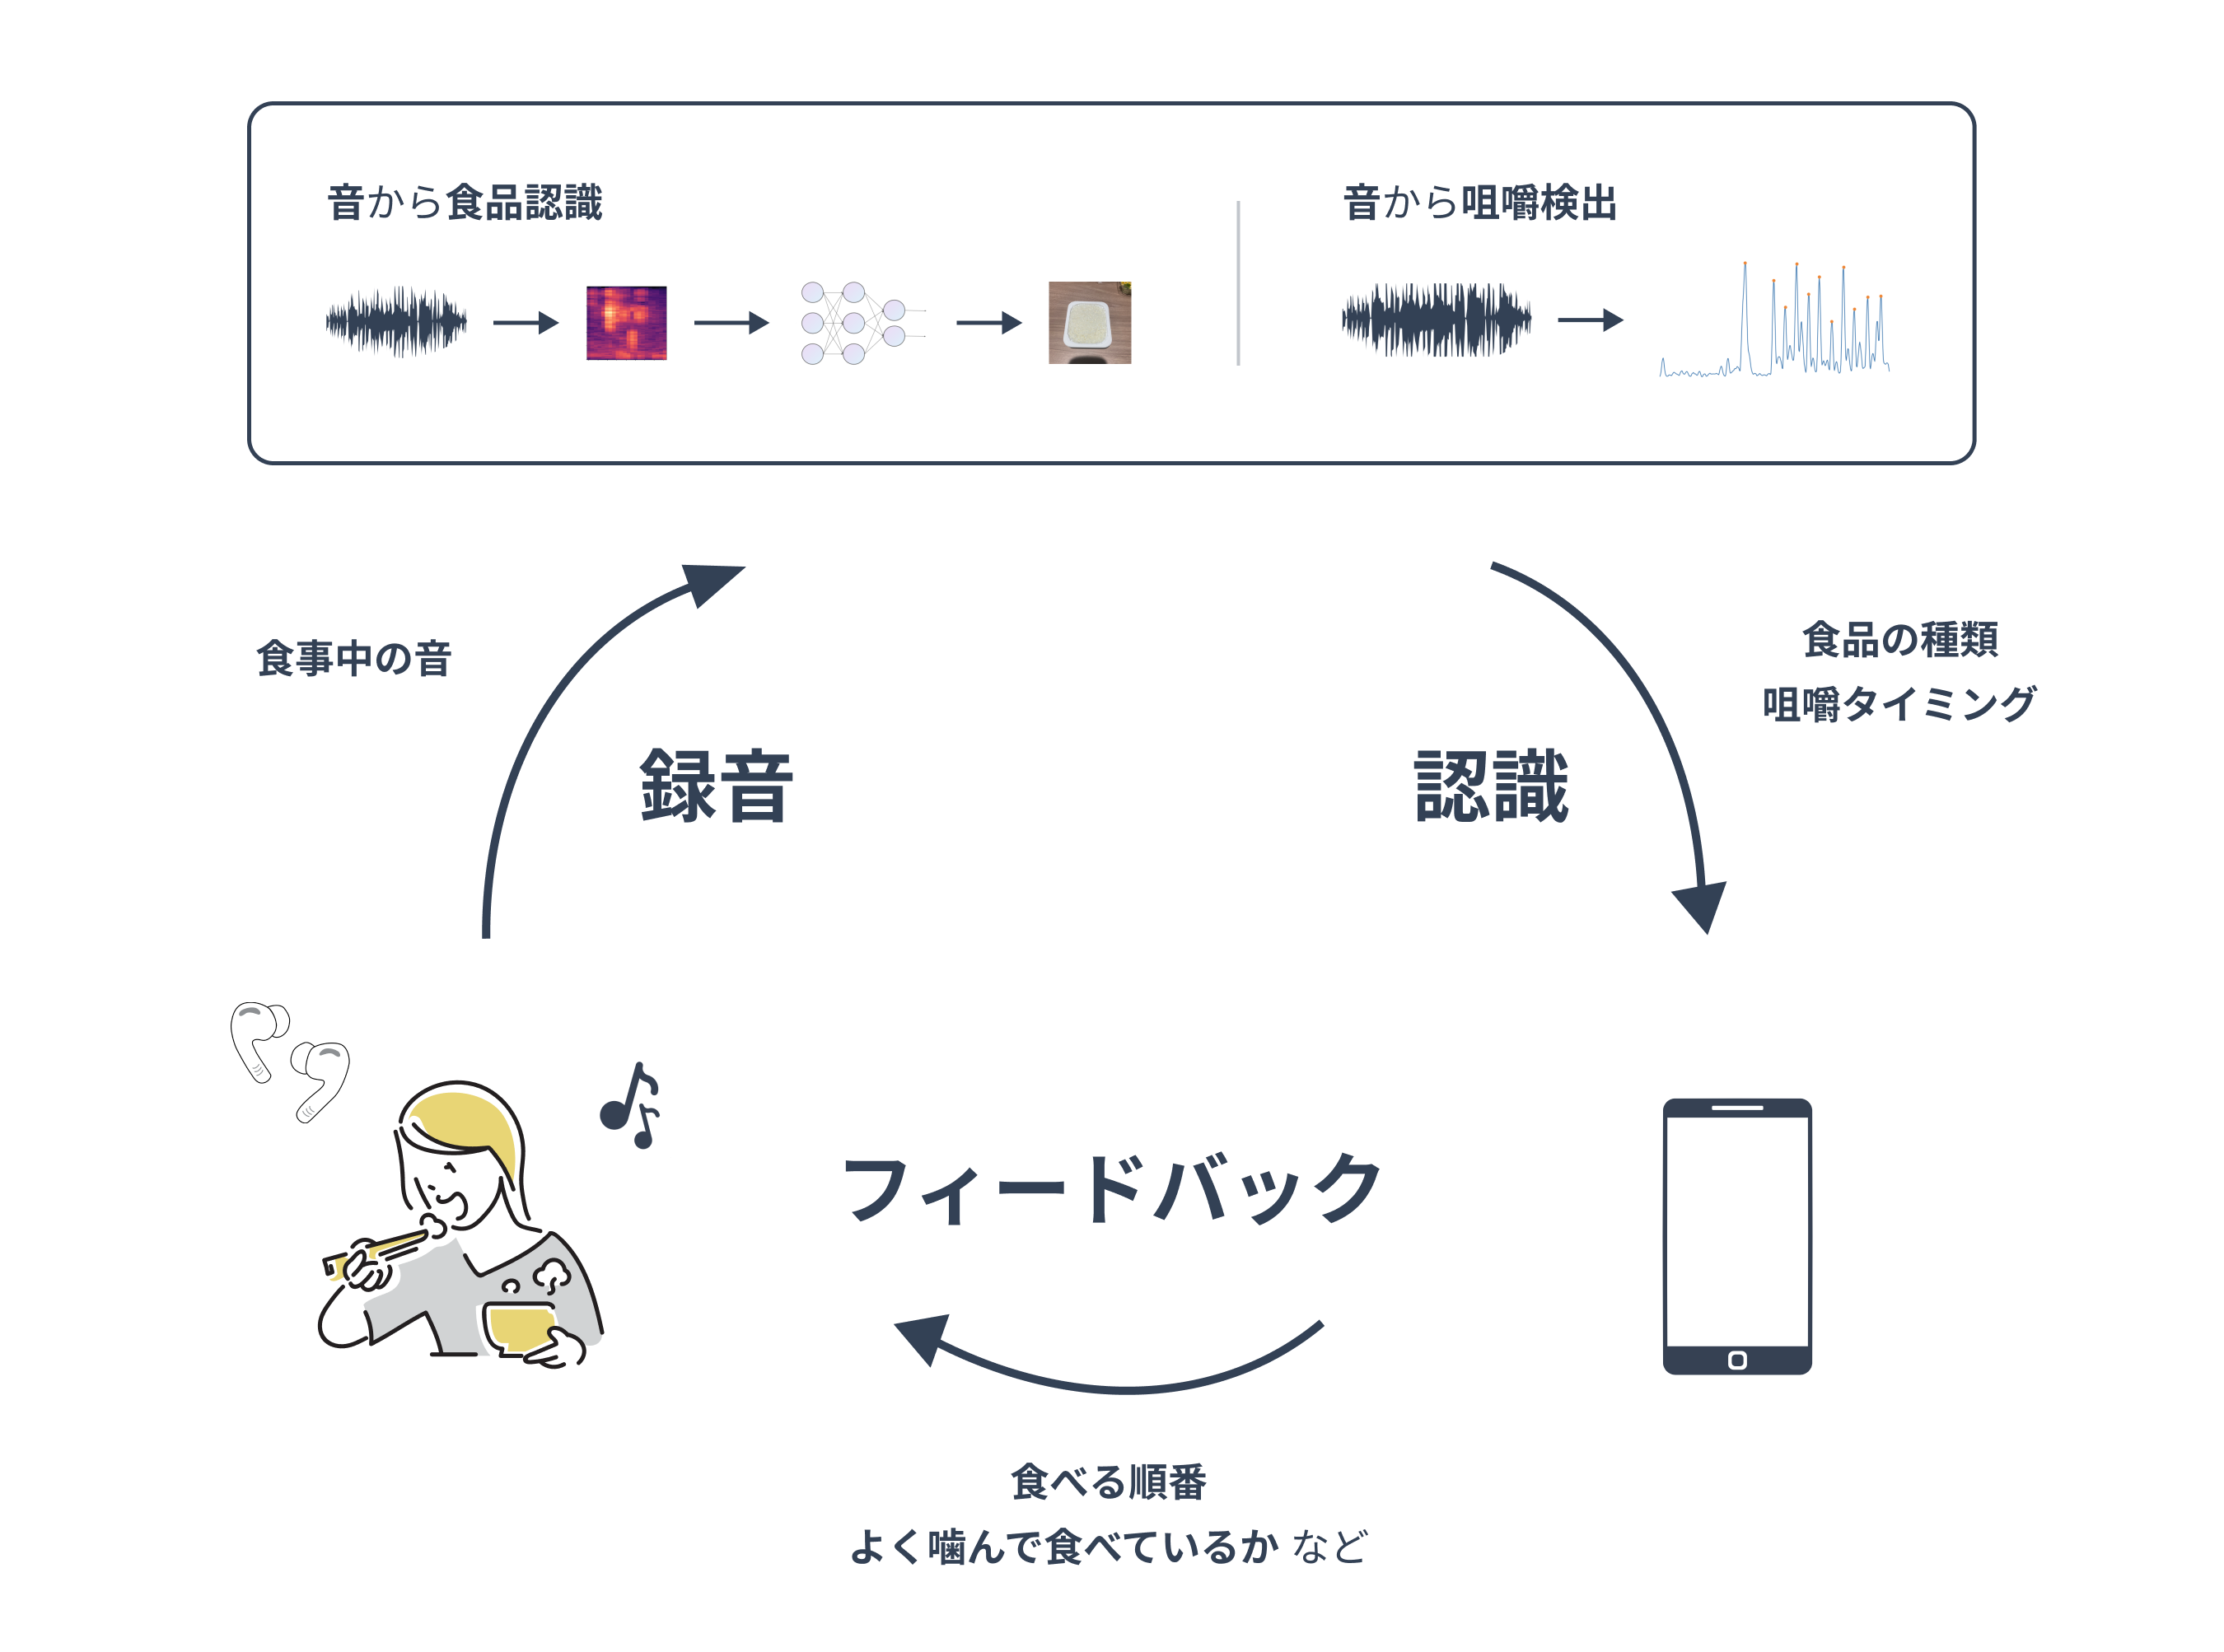
\includegraphics[clip,  width=1.0\hsize]{img/system.png}
    \caption{食事中の音を分析するための計測システムの提案}
    \label{fig:system}
  \end{center}
\end{figure}
%%%%%%%%%%%%%%%%%%%%%%%%%%%%%%%%%%%%%%%%%%%%%%%%

食べる順番や速度などを含む食事行動の記録に着目した研究や技術も存在する. シャープが開発したbitescan\footnote{咀嚼計「bitescan(バイトスキャン)」:シャープ~\url{https://jp.sharp/business/bitescan/}}では, 独自の耳掛け式のウェアラブルデバイスを用いて, 食事中にリアルタイムで咀嚼回数を計測することで, 咀嚼テンポや食事の時間などを記録することができる. しかし, 独自のウェアラブルデバイスが必要となるため, 誰でも利用できるアプリケーションに組み込むことは難しく, そもそも咀嚼回数のみを計測しているため, 食べる順番を記録することができない. また, 食べる順番や速度などをアドバイスするために, ウェアラブルデバイスで食事行動を撮影した一人称映像から食事内容をリアルタイムで検出する研究も存在する\cite{10.1145/3551626.3564964}. しかし, この手法も食事中にカメラで撮影し続ける必要があるため, 一般的な食事シーンで計測を行うのは受け入れ難い.

我々の研究グループでは, 健康的な食生活を促進する行動変容支援システムとしてeat2picを提案している\cite{10.1145/3580784}. しかし, eat2picのセンシングアプローチは, カメラとIMUを搭載した専用の箸型センサを使用する必要があるため, 日常生活での利便性や社会全体への普及可能性という観点で, 課題が残っている. それに対して, 本研究ではすでに普及している市販のイヤラブルデバイスとスマートフォンのみを使用し, 食事内容と咀嚼回数の推定が可能なセンシング手法を提案する. 本稿では, 図\ref{fig:system}に示すように, 食事中に発生する音を収集し, 収集したデータを分析し, 食事内容と咀嚼回数の推定を行う一連の設計について述べる. 図\ref{fig:system}では, 計測・分析・可視化というステップを示しているが, 本稿では計測・分析のみを行い, 可視化については本稿では取り扱わない. 具体的には, 食事中の音をワイヤレスイヤホンで録音しつつ, 被験者自身が咀嚼回数をカウントできる独自のアプリケーションを開発し, このアプリケーションを用いてデータ収集を行う. 分析については, 計測した食事中の音をメルスペクトログラムに変換し, 畳み込みニューラルネットワークで学習させ, 食事内容推定モデルの作成を行う. また, メルスペクトログラムの各時間軸毎の全ての周波数の信号強度の平均をとり, ピーク検出を行うことで咀嚼の検出を行う. データ収集実験では, 15名の被験者を対象にアプリケーションを配布し, ワイヤレスイヤホンを装着した状態で, 一品ずつ食事を行った. また, 咀嚼検出の分析のために, 実験中に被験者自身の咀嚼回数をカウントするように指示した. 16種類の食品に対して録音を行い, 合計で13422秒の音データを得られた. その結果, 収集した音データで食事内容推定モデルを学習させたところ, 検証用の音データに対して, 精度$77.5\%$で食事内容を推定できることを確認した. また, 10秒間の音データに対して被験者がカウントした咀嚼回数とピーク検出回数との間の平均絶対値誤差$MAE$を算出したところ, $MAE = 4.9$を確認することができた.

本稿の構成は以下の通りである.
第2章で食事内容の推定に関する関連研究について述べる. 第3章でデータ収集アプリケーションの設計・開発について述べ,第4章で食事中の音から食事内容・咀嚼回数を推定する手法について述べる. 第5章で評価実験について述べ,最後に第6章で本稿の結論および今後の課題について述べる.
